\section{Algoritma Code Generation Lokal}

Untuk menghasilkan kode di dalam sebuah \textit{Basic Block}, kompilator menggunakan algoritma yang memaksimalkan pemanfaatan register melalui informasi lokal.

\subsection{Informasi Penggunaan Berikutnya (Next-Use Info)}
Kompilator melakukan pemindaian mundur (\textit{backward scan}) pada blok tersebut untuk menentukan kapan sebuah variabel akan digunakan lagi. Informasi ini disimpan di dalam tabel simbol atau anotasi pada instruksi.
\begin{itemize}
    \item Jika variabel \code{x} digunakan di baris $i$ dan tidak digunakan lagi setelah itu di dalam blok tersebut, maka register yang menampung \code{x} dapat langsung dibebaskan atau digunakan untuk menampung hasil operasi di baris $i$.
    \item Informasi ini sangat vital bagi fungsi \code{GetReg()} untuk meminimalkan pengosongan register ke memori (\textit{spilling}).
\end{itemize}

\subsection{Fungsi Pembantu GetReg}
Fungsi \code{GetReg(I)} dipanggil untuk setiap instruksi $I: x = y \ op \ z$ untuk menentukan register mana yang akan menampung $x$. Aturannya antara lain:
\begin{enumerate}
    \item Jika variabel $y$ sudah berada di register $R$, dan $y$ tidak memiliki penggunaan lagi setelah instruksi ini (\textit{no next use}), maka $R$ dapat digunakan untuk menampung hasil $x$.
    \item Jika tidak ada register kosong, pilih register yang variabel di dalamnya memiliki "jarak penggunaan berikutnya" paling jauh (\textit{Heuristic: Farthest Next Use}).
\end{enumerate}

\begin{figure}[!htbp]
    \centering
    \adjustbox{max width=0.8\textwidth,center}{%
    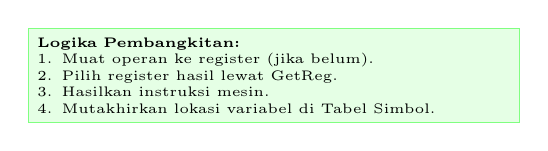
\begin{tikzpicture}[
        rect/.style={rectangle, draw=green!50, fill=green!10, text width=6cm, font=\tiny}
    ]
    \node[rect] (gen) {
        \textbf{Logika Pembangkitan:}\\
        1. Muat operan ke register (jika belum).\\
        2. Pilih register hasil lewat GetReg.\\
        3. Hasilkan instruksi mesin.\\
        4. Mutakhirkan lokasi variabel di Tabel Simbol.
    };
    \end{tikzpicture}%
    }
    \caption{Alur Kerja Code Generator di tingkat Basic Block}
\end{figure}
